\documentclass[a4paper,12pt]{article}
\parindent 0pt
\parskip 1mm
\usepackage{amsmath}
\usepackage[dvips]{epsfig}

\begin{document}

\begin{center}

{\Large\bf CN 510 - Principles and Methods of Cognitive and Neural Modeling}

\bigskip

{\large\bf Assignment \# 5}
\smallskip

{\large\bf John Joseph}
\end{center}

\bigskip
{\bf Recurrent Competitive Fields}
\bigskip

This week's assignment focuses on the dynamics of recurrent competitive fields, and has us plot and analyze the impact of the signalling function on the model. We solve the differential equation

\begin{equation}
  \frac{dx_i}{dt} = -Ax_i+(B-x_i)[f(x_i)+I_i] - x_i\sum\limits_{j \neq i} f(x_j)
\end{equation}

Where $I$ represents the input upon neuron $x_i$ for the $i^{th}$ of $n$ neurons. $n=10$, and the inputs and initial values for $x$ are provided. We are also provided the constants A=1,B=3, as well as the parameter F=0.25. 

\vspace{2mm}

$F$ is a parameter of the signalling function $f(x)$. We will use four separate signalling functions:

\begin{equation}
f(x)=w
\end{equation}

\begin{equation}
f(x)=w^2
\end{equation}

\begin{equation}
f(x)=\frac{w}{F+w}
\end{equation}

\begin{equation}
f(x)=\frac{w^2}{F+w^2}
\end{equation}

The functions are known as Linear, Faster-than-Linear, Slower-than-Linear, and Sigmoidal (respectively). 

\vfil\eject

{\bf Part A}

In Part A we initialize every $x$ to 0 and turn the current on for the first second only. Some analysis can be done to give us an idea of what to expect, and for the most part I felt pretty good about my results. 

\bigskip
{\bf Linear}
\bigskip
\begin{figure}[h!]
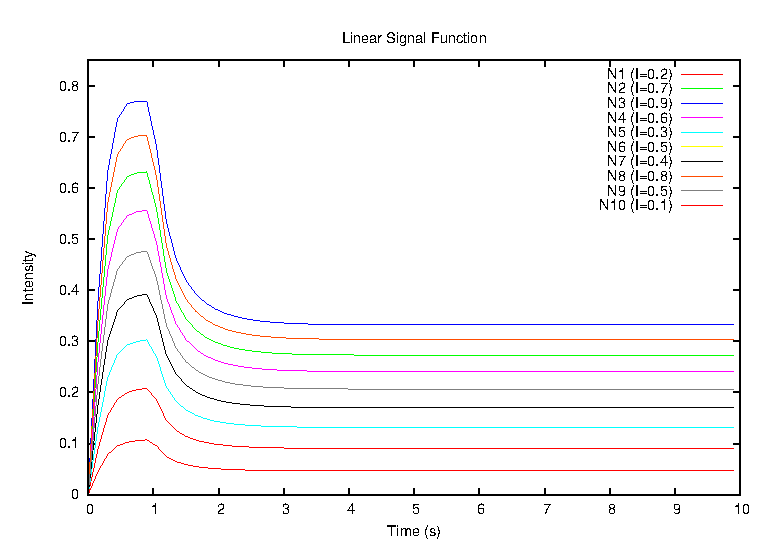
\epsfig{file=data/figures/partA/linearTime,width=8cm,height=6cm}
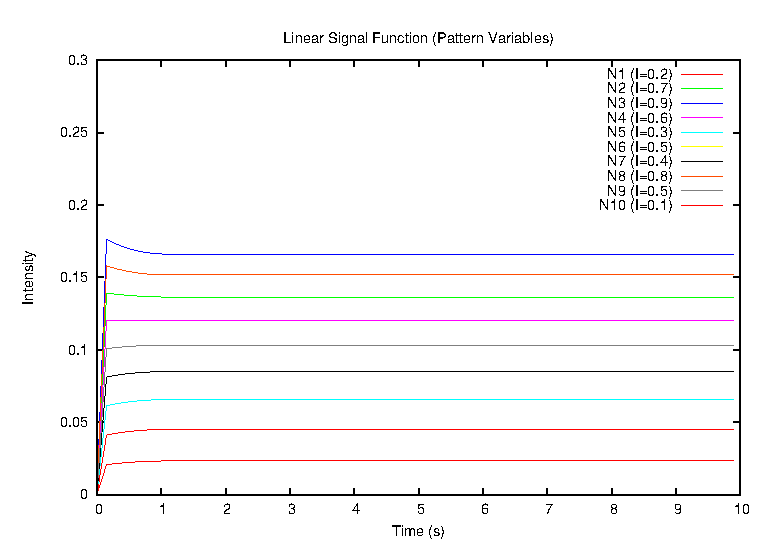
\epsfig{file=data/figures/partA/linearTimeP,width=8cm,height=6cm}
\end{figure}

\begin{figure}[h!]
\begin{center}
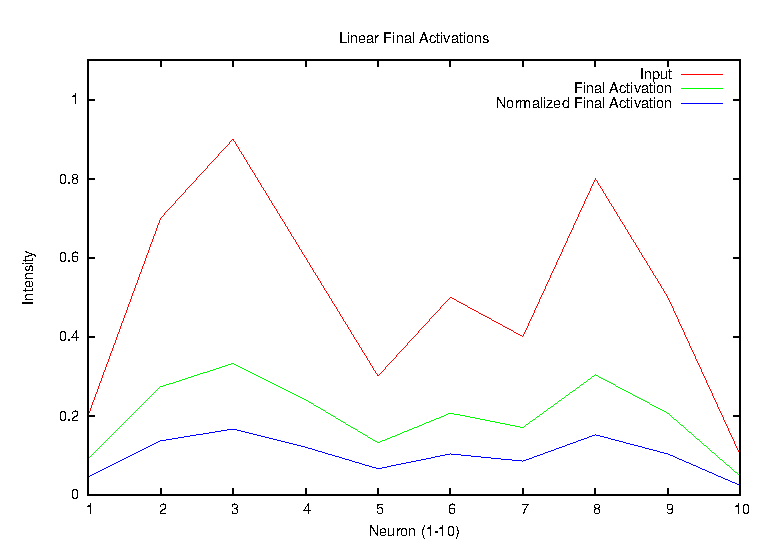
\epsfig{file=data/figures/partA/linearFinal,width=12cm,height=9cm}
\end{center}
\end{figure}

\vfil\eject

It seemed pretty clear to me that, though there was a significant amount of attenuation, the overall pattern was well preserved. You can see in the time-dependent plots on top that the lines were essentially parallell throughout, and in the equilbrium plot there is a visible retention of the original input. 

\vspace{2mm}

The pattern variables displayed similar behavior, although their values were obviusly lower due to the ``normalization'' of the network. It is also worth commenting on the strange jumpiness that occurs during the initial second; I could attribute this either to computational error on my part or initial instabilities. Regardless, it seems as though the pattern variable plot responded differently because of how large the values got in this first second, making them much lower in value right from the start. 

\bigskip

{\bf Faster-than-Linear}

\bigskip

The faster than linear plot showed the behavior that was described in the notes to a tee, favoring heavily neuron three once the solution converges. This is because neuron three received the largest input, and the Faster-than-Linear function leads to a ``winner take all'' situation where the strongest input dominates. In the unnormalized plot we see the neuron surpass its input value and obtain a value of around $2.5$, which shows up later in the Slower-than-Linear plot. 

\vspace{2mm}

In the pattern variable plot, neuron three obtained a value of 1. This is the highest value attainable, and shows that the other neurons have decayed to zero. This happens fairly soon after the input is turned off in both cases, though again the higher values in the non-normalized plot cause the pattern variables to start off at much lower values. 

\begin{figure}[h!]
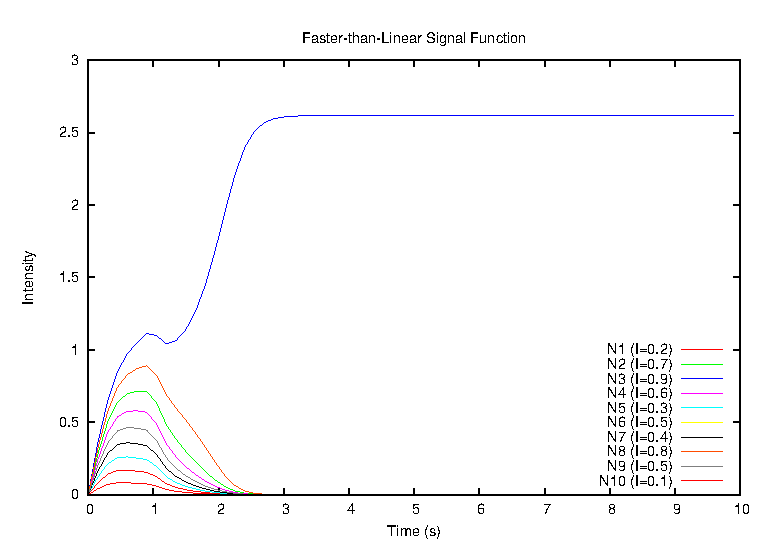
\epsfig{file=data/figures/partA/fastTime,width=8cm,height=6cm}
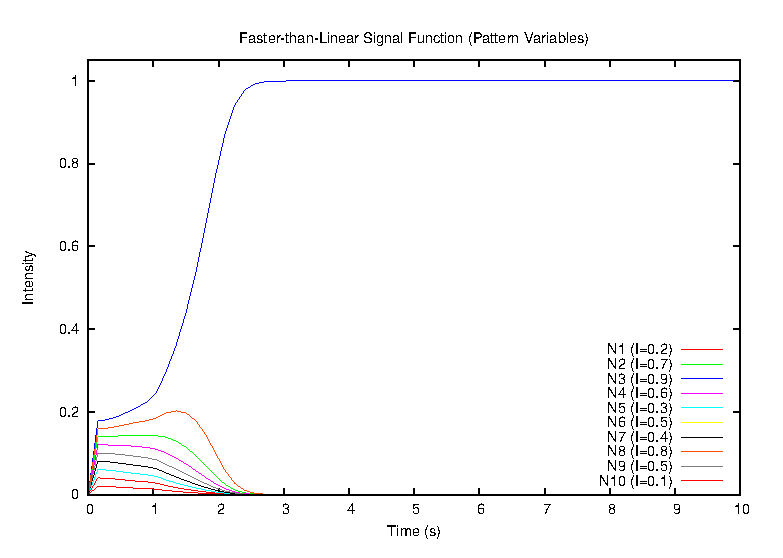
\epsfig{file=data/figures/partA/fastTimeP,width=8cm,height=6cm}
\end{figure}

\begin{figure}[h!]
\begin{center}
\epsfig{file=data/figures/partA/fastFinal,width=12cm,height=9cm}
\end{center}
\end{figure}

\bigskip

{\bf Slower-than-Linear}

\bigskip

I wasn't entirely sure, but if what I took from the notes was correct then my Slower-than-Linear plot behaved alright. The neurons all converged to the same value of 2.5 fairly quickly. At first I thought this was a bug in my code, but I created an animation in OpenGL and watched the inputs all flatten out at 2.5. 

\vspace{2mm}

The inputs did climb during the initial second, even somewhat in the pattern variable plot. However it did not take long for things to start decaying, and by about the $3^{rd}$ second the neurons had all decayed to zero. 

\begin{figure}[h!]
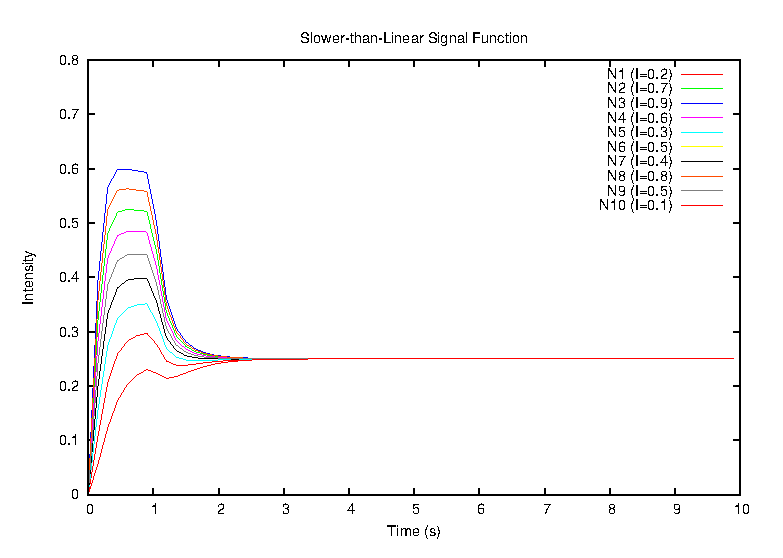
\epsfig{file=data/figures/partA/slowTime,width=8cm,height=6cm}
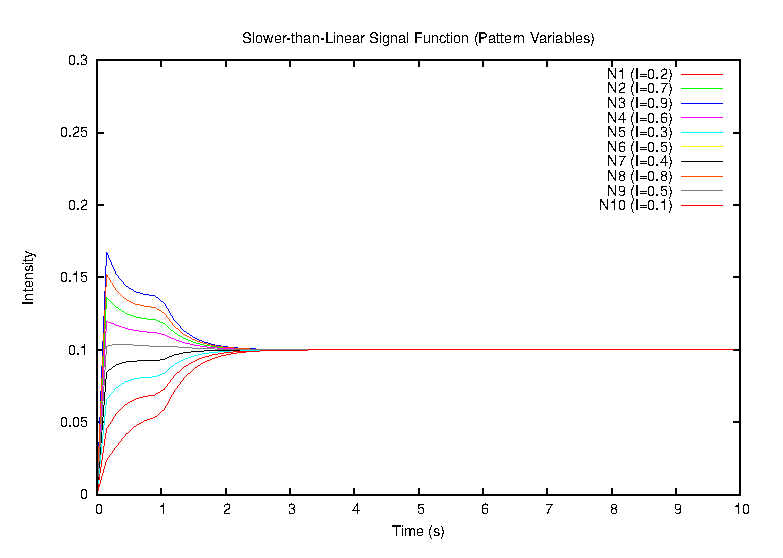
\epsfig{file=data/figures/partA/slowTimeP,width=8cm,height=6cm}
\end{figure}

\begin{figure}[h!]
\begin{center}
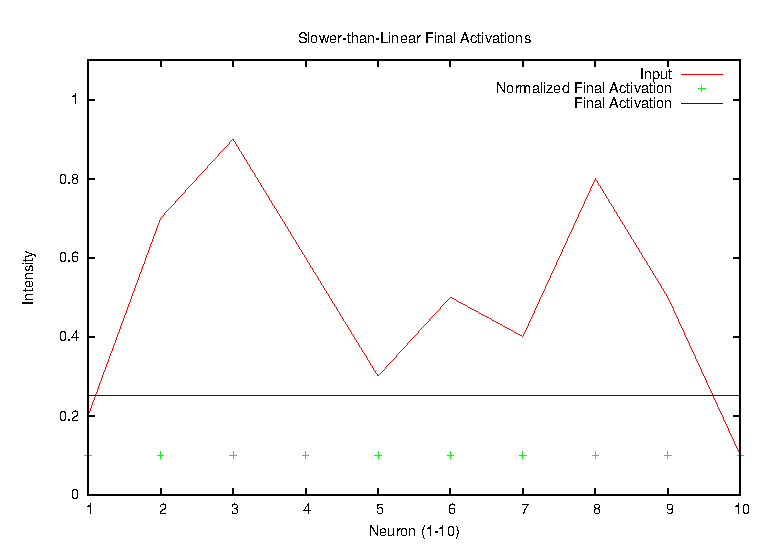
\epsfig{file=data/figures/partA/slowFinal,width=12cm,height=9cm}
\end{center}
\end{figure}

\vfil\eject

{\bf Sigmoidal}

\bigskip

The sigmoidal plot also behaved rather nicely, preserving only values whose inputs passed a certain threshold. These neurons, 2,3, and 8, were the three highest inputs by a sizeable margin, and the neurons whom they left behind soon feel to zero. 

\vspace{2mm}

In the pattern variable plot still shows the same behavior, and though its values are significantly smaller it does managed to keep up a big longer than the non-normalized neurons did. I'm not entirely sure what that means, but one can cleraly see from the plots that are strongest inputs are the only ones that survive. 

\begin{figure}[h!]
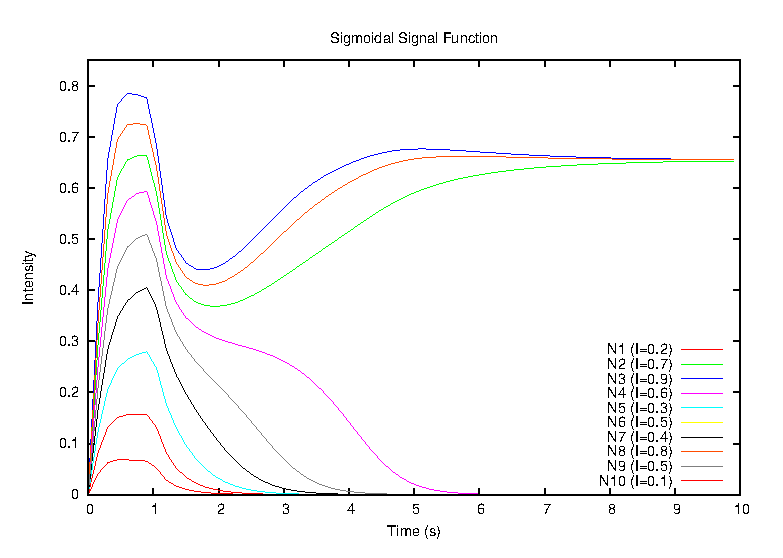
\epsfig{file=data/figures/partA/sigTime,width=8cm,height=6cm}
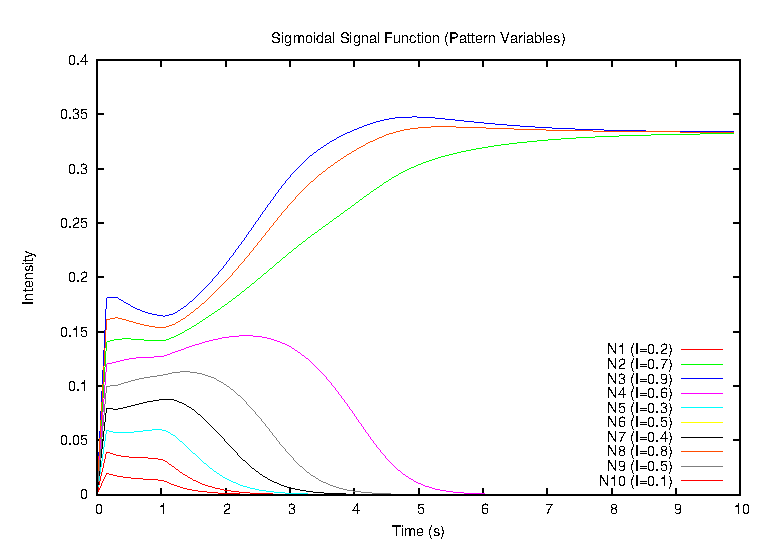
\epsfig{file=data/figures/partA/sigTimeP,width=8cm,height=6cm}
\end{figure}

\begin{figure}[h!]
\begin{center}
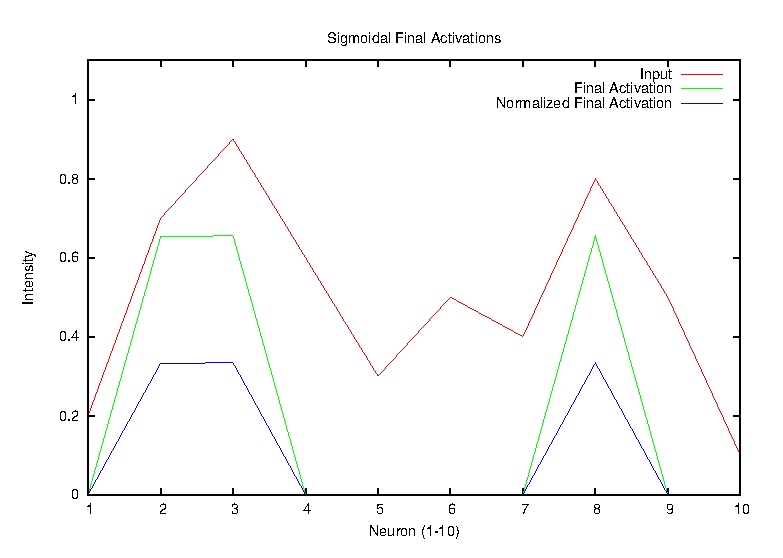
\epsfig{file=data/figures/partA/sigFinal,width=12cm,height=9cm}
\end{center}
\end{figure}

\vfil\eject

{\bf Part B}
\bigskip

Part B is the same as part A, except are neurons are now initialized to a set of given values. It is here that I was unsure whether or not my neurons were behaving correctly, but in the long run I rarely found much difference in the results.

\vspace{2mm}



The differing inputs caused the neurons to start out at different places, but it didn't take long for the neurons to fall into a behavior that was very reminiscent of those from part A. In fact, there were several times when I was unable to distinguish the final activation plots of part A and part B, because they come out to be the same thing. 

\vspace{2mm}

My only concern was that the initial values caused my already jumpy initial second to further exhibit strange behavior. Perhaps if I had chosen a smaller time step (I used 0.05) this could have been avoided, but in general the behavior of this part was analagous to what had happened in part A. 

\bigskip
{\bf Linear}
\bigskip

The linear plots did not misbehave, and the aforementioned strangeness during second 1 soon vanishes as it did before. As I mentioned, the final activation plot of these neurons as often indistinguishable from that of part A, and this was no exception. 

\begin{figure}[h!]
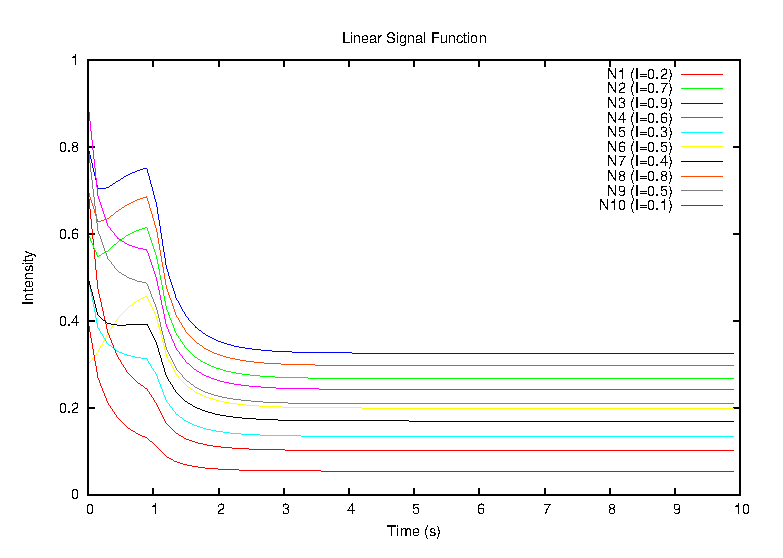
\epsfig{file=data/figures/partB/linearTime,width=8cm,height=6cm}
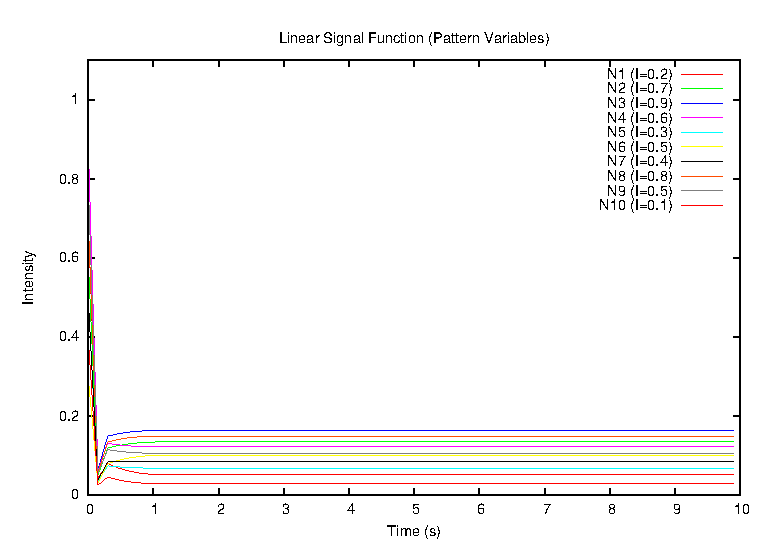
\epsfig{file=data/figures/partB/linearTimeP,width=8cm,height=6cm}
\end{figure}

\begin{figure}[h!]
\begin{center}
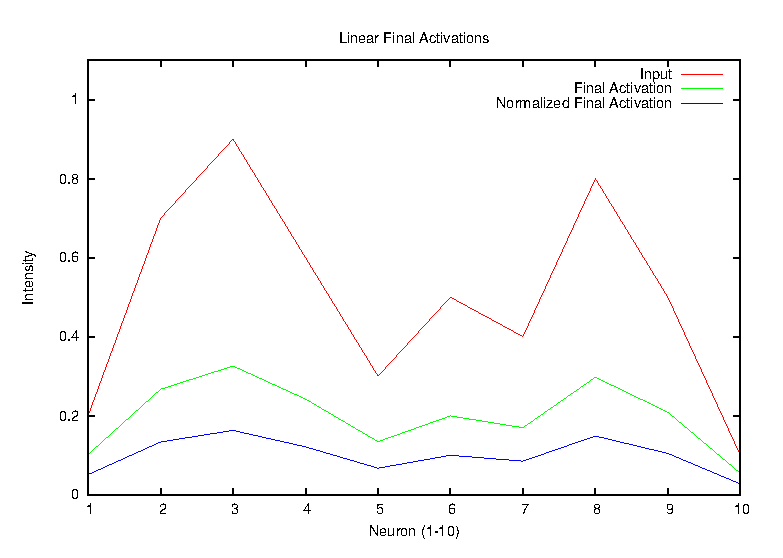
\epsfig{file=data/figures/partB/linearFinal,width=12cm,height=9cm}
\end{center}
\end{figure}

\vfil\eject

\bigskip
{\bf Faster-than-Linear}
\bigskip

Faster-than-Linear behaved as we'd expect, and all neurons save for 3 are pulled from their initial values down to zero. There is a noticeable bump in the pattern variable plot during the very early stages of the simulation, which I attribute to the very small sum terms the system had combined with the sharp gradient we see in the plot. As with before, the final plots are indistinguishable and the $3^{rd}$ pattern variable goes to 1. 

\begin{figure}[h!]
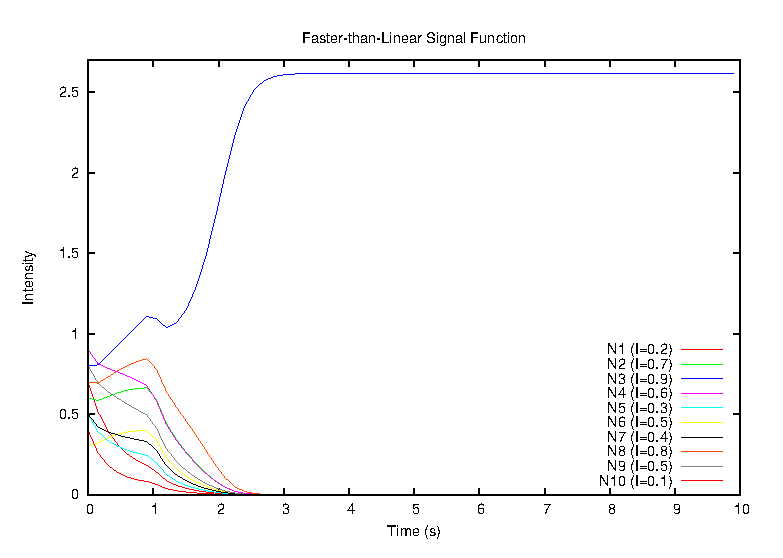
\epsfig{file=data/figures/partB/fastTime,width=8cm,height=6cm}
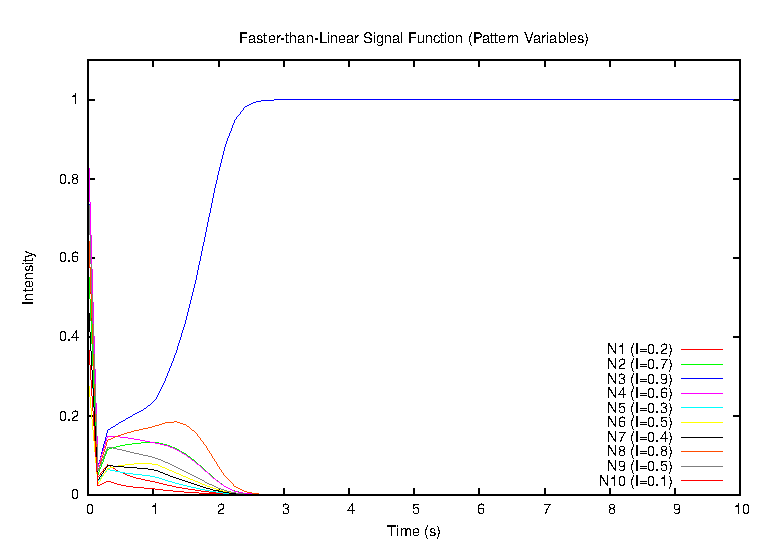
\epsfig{file=data/figures/partB/fastTimeP,width=8cm,height=6cm}
\end{figure}

\begin{figure}[h!]
\begin{center}
\epsfig{file=data/figures/partB/fastFinal,width=12cm,height=9cm}
\end{center}
\end{figure}

\bigskip
{\bf Slower-than-Linear}
\bigskip

Slower-than-Linear behaves as expected, with the unnormalized values going to 2.5. The normalized values go to 0.1, which is expected as Slower-than-Linear brings the system to uniformity. 

\begin{figure}[h!]
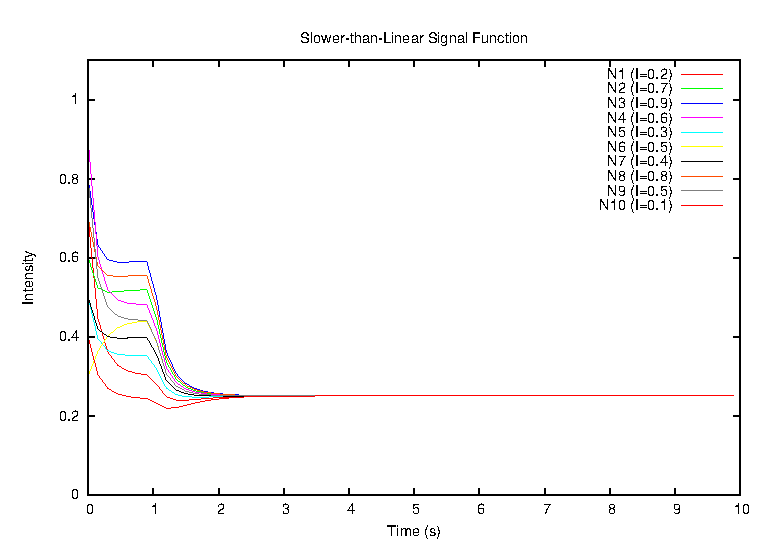
\epsfig{file=data/figures/partB/slowTime,width=8cm,height=6cm}
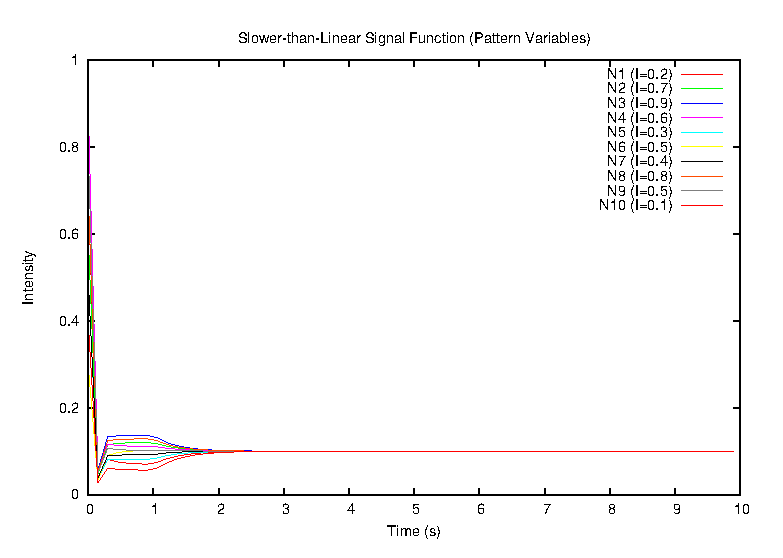
\epsfig{file=data/figures/partB/slowTimeP,width=8cm,height=6cm}
\end{figure}

\begin{figure}[h!]
\begin{center}
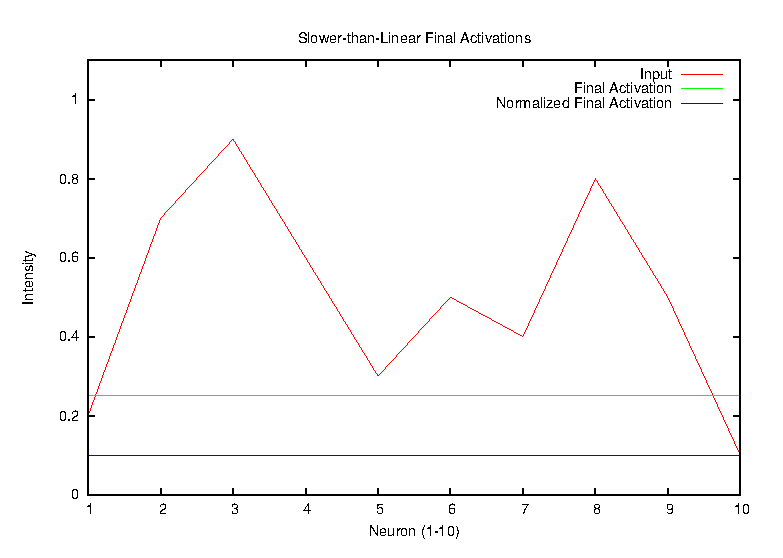
\epsfig{file=data/figures/partB/slowFinal,width=12cm,height=9cm}
\end{center}
\end{figure}

\vfil\eject

\bigskip
{\bf Sigmoidal}
\bigskip

The sigmoidal plots were also the same, which I suppose I should have expected. I anticipated that the inputs would throw this one off somehow and perhaps bring in or take out one of the chosen values from before. However, it seems as though there was no difference in outcomes, and neurons 2,3, and 8 were again favored. As a sidenote, I thought the plots were rather nice to look at. 

\begin{figure}[h!]
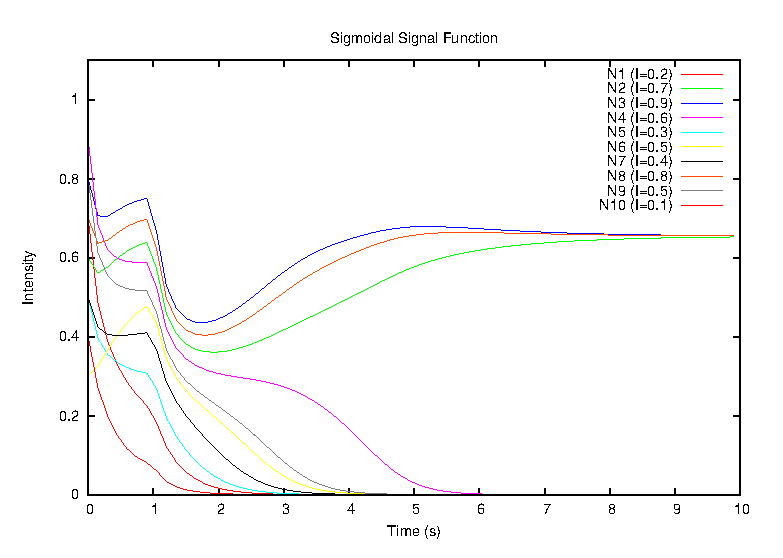
\epsfig{file=data/figures/partB/sigTime,width=8cm,height=6cm}
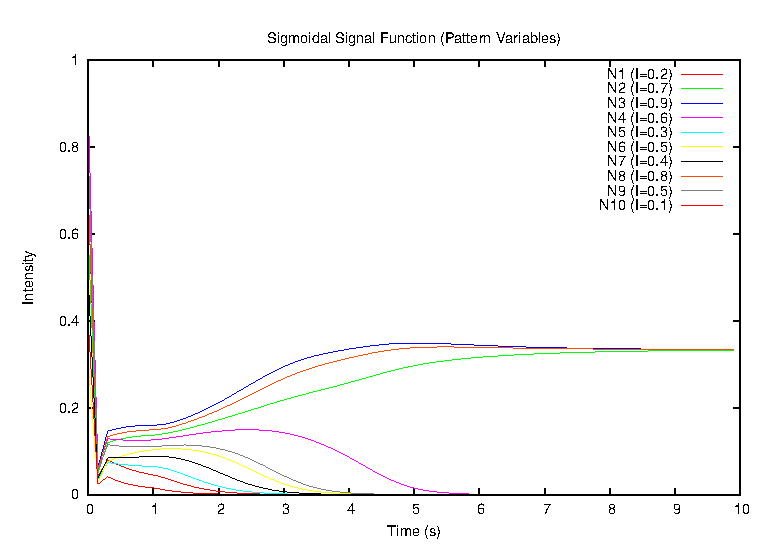
\epsfig{file=data/figures/partB/sigTimeP,width=8cm,height=6cm}
\end{figure}

\begin{figure}[h!]
\begin{center}
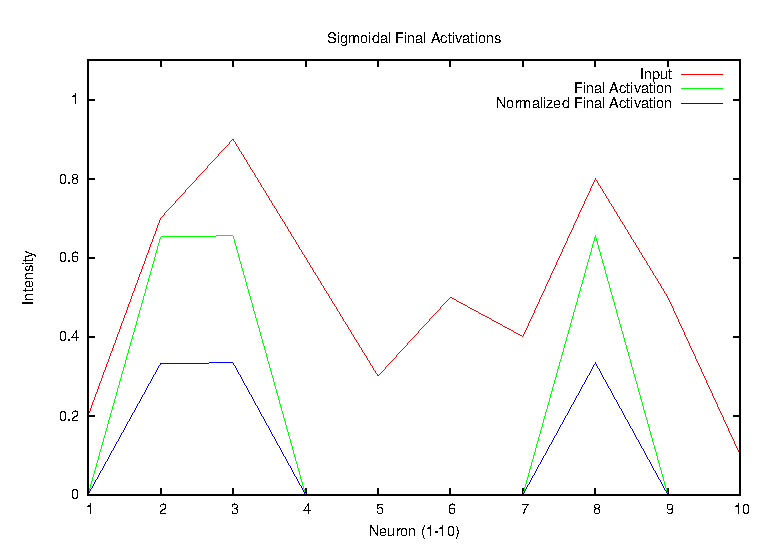
\epsfig{file=data/figures/partB/sigFinal,width=12cm,height=9cm}
\end{center}
\end{figure}

\vfil\eject
\bigskip
{\bf Conclusions}
\bigskip

Overall I thought things went pretty well. My plots could have been a lot more inaccurate, and despite some errors regarding the initial second my neurons seemed pretty well behaved. 

\vspace{2mm}

In general the initial conditions of the problem had little impact on its long-term solution, and the dependency upon the signal function of the final activations was quite similar to what was described in class. 

\bigskip
\bigskip
\bigskip
\bigskip
\bigskip
\bigskip
\bigskip
\bigskip
\bigskip
\bigskip
\bigskip
\bigskip
\bigskip
\bigskip
\bigskip
\bigskip
\bigskip
\vfil\eject
Here is the do-while loop I used to carry out my time simulation. 

\bigskip
\begin{verbatim}
// loop variable and current sums
int i,k,count=0,printRate=2;
T Xsum,t=0,X=0;

do {
    Xsum=0;
    // Fill up the sum term
    for (k=0;k<N;k++)
      Xsum+=sigFunc(F,x[k]);
    T a,b;
    for (i=0;i<N;i++)
      { //Solve the equation
        a=(-A-I[i]-Xsum);
        b=B*(sigFunc(F,x[i])+I[i]);
        x[i]=solveRK(x[i],a,b);
      }  
    count++;
    t+=DT;
    if (count%printRate==0)
      {
         for (i=0;i<N;i++)
         X+=x[i];
         count=0;

        //Here we would output to our files

         X=0;
      }
  } while (t<=1); 
\end{verbatim}

Where we would continue the same loop for $t=[1,10]$ but exclude the I term, thus ``turning off'' our input. 

\end{document}
